\chapter{Hybrid Generative and Discriminative models}

\section{Energy-Based Models}\label{EBM}
Energy-based models (EBM) was firstly introduced here \cite{energy}, but following nomenclature was established here \cite{energy2}. EBM assume that probability densities $p(\boldsymbol{x})$ for $\boldsymbol{x} \in \mathbb{R}^D$ can be expressed in the form
\begin{equation}
	p_{\boldsymbol{\theta}}\left(\boldsymbol{x}\right) = \frac{\exp\left(-E_{\boldsymbol{\theta}}(\boldsymbol{x})\right)}{Z(\boldsymbol{\theta})},
\end{equation}
where function $E_{\boldsymbol{\theta}} : \mathbb{R}^D \to \mathbb{R}$ is called Energy and maps each datapoint $\boldsymbol{x}$ to a scalar. The denominator $Z(\boldsymbol{\theta})$ is a normalization constant (also known as partition function), thus
\begin{equation}
	Z(\boldsymbol{\theta}) = \sum_{i=1}^N \exp\left(-E_{\boldsymbol{\theta}}(\boldsymbol{x}_i)\right),
\end{equation}
where  the summation is over all datapoints $\boldsymbol{x}$ available. The sum turns into integral for a continuous $\boldsymbol{x}$.   Very important observations made authors in \cite{energy2}, where they show, that classifiers in supervised learning are secretly energy-based models on $p(\boldsymbol{x},y)$ and can be expressed as
\begin{equation}
	p\left(\boldsymbol{x},y\right) = \frac{\exp\left({f_{\boldsymbol{\theta}}\left(\boldsymbol{x}\right)[y]}\right)}{Z(\boldsymbol{\theta})}.
\end{equation}
The objective above is called joint energy model and it is obvious that $f_{\boldsymbol{\theta}}\left(\boldsymbol{x}\right)[y] = -E_{\boldsymbol{\theta}}(\boldsymbol{x},y)$. It may come in handy to have only a density model of datapoints $p(\boldsymbol{x})$ without labels. This could be achieved by marginalizing $p(\boldsymbol{x},y)$ over $y$ 
\begin{equation}
	p\left(\boldsymbol{x}\right) = \frac{\sum_{i=1}^C\exp\left({f_{\boldsymbol{\theta}}\left(\boldsymbol{x}\right)[y_i]}\right)}{Z(\boldsymbol{\theta})},
\end{equation}
where energy is given by $E_{\boldsymbol{\theta}}(\boldsymbol{x}) = -\log\sum_{i=1}^C\exp\left({f_{\boldsymbol{\theta}}\left(\boldsymbol{x}\right)[y_i]}\right)$. Very useful property appears when computing $p(y|\boldsymbol{x})$. We can take advatage of the definition of conditional distribution $p(y|\boldsymbol{x})~=~\frac{p\left(\boldsymbol{x},y\right)}{p\left(\boldsymbol{x}\right)}$, yielding  
\begin{equation}\label{softmaxdef}
	p_{\boldsymbol{\theta}}\left(y|\boldsymbol{x}\right) = \frac{\exp\left({f_{\boldsymbol{\theta}}\left(\boldsymbol{x}\right)[y]}\right)}{\sum_{i=1}^C\exp\left({f_{\boldsymbol{\theta}}\left(\boldsymbol{x}\right)[y_i]}\right)}.
\end{equation}
Note that the normalization constant $Z(\boldsymbol{\theta})$ canceled out and we ended up with the same function, which was introduced in \eqref{softmax}. 
\section{Contrastive learning}
 Contrastive learning \cite{contrastive1, contrastive2} is a ML technique used to learn so-called general features of a dataset by teaching the model which datapoints are similar or different. This all happens without labels, therefore contrastive learning is often called \emph{self--supervised} technique of ML.  In contrastive learning problems, it is very usual to optimize an objective often called contrastive loss, which can be written in the form as follows
\begin{equation}\label{eq:contrastive}
	\min_{\boldsymbol{\theta}}- \mathbb{E}_{p_{\mathrm{data}}(\boldsymbol{x})}\left[\log \frac{\exp\left({h_{\boldsymbol{\theta}}\left(\boldsymbol{x}\right)\cdot h_{\boldsymbol{\theta}}\left(\boldsymbol{x}'\right)}\right)}{\sum_{i=1}^N\exp\left({h_{\boldsymbol{\theta}}\left(\boldsymbol{x}\right)\cdot h_{\boldsymbol{\theta}}(\boldsymbol{x}_i) }\right)} \right].
\end{equation}
Function $h_{\boldsymbol{\theta}}: \mathbb{R}^D \to \mathbb{R}^H$ maps each data point to a representation space with dimension $H$, while $\boldsymbol{x}$ and $\boldsymbol{x}'$ are two different augmented views of the same data point. If $\boldsymbol{x}$ is an image, then augmented view of $\boldsymbol{x}$ can be obtained for example by rotation or colorization of that image. Note that the inner product between two vectors can replaced with any distance metric, for example Euclidean distance. \\
What this objective does is that it tries to maximally distinguish an input $\boldsymbol{x}_i$ from an alternative input $\boldsymbol{x}'_i$. In other words, \eqref{eq:contrastive} reduces the distance between representations of different augmented views of the same image $\boldsymbol{x}, \boldsymbol{x}'$ (positive pairs) and increases the distance between representations of augmented views of from different images (negative pairs). This means that the model should be able to distinguish between different types of images without even knowing what these images really are. 

\section{Noise--contrastive estimation}
Suppose one has to estimate a model that is specified by an non-normalized probability den-
sity function $q^0_{\bt}\left(\boldsymbol{x}\right)$. In such case, one can utilize noise--contrastive estimation (NCE). The first step is to  introduce the another parameter c among the estimated parameters $\bt$. For clarity, the symbol $\bt^\star=\left\lbrace\bt,c\right\rbrace$ is introduced for the set of estimated parameters including
c. Using this notation, the following equalities hold
\begin{align}
    q_{\bt^\star}\left(\boldsymbol{x}\right)
    \end{align}
which means that the newly introduced parameter c is an estimate of the negative logarithm of
the normalization constant $Z\left(\bt\right)$.
As the name of the subsection suggests, we use noise to estimate. By our convention, let $\bx_1,\bx_2,\dots,\bx_N$
be the observations and $\boldsymbol{e}_1,\boldsymbol{e}_2,\dots,\boldsymbol{e}_N$ be the artificially generated noise data with known distribution $\psi\left(\bt\right)$. The $\widehat{\bt^\star}$ estimate is then defined as
\begin{align}
    \widehat{\bt^\star} &= \argmax_{\bt^\star} \pazocal{L}^{\mathrm{NC}}\left(\bt^\star\right)\\
   &= \argmax_{\bt^\star} \frac{1}{2N}\sum_{i=1}^N \ln\sigma_{\bt^\star}\left(\bx_i\right) + \ln\left(1-\sigma_{\bt^\star}\left(\boldsymbol{e}_i\right) \right)\label{NCEloss}
\end{align}
where $\sigma_{\bt^\star}$ is logistic function
\begin{align}
\sigma_{\bt^\star} = \frac{1}{1 + \exp\left(-G_{\bt^\star}\left(\bx\right) \right)}
\end{align}
and finally, function $G_{\bt^\star}$ represents the difference of the log-likelihoods of $q_{\bt^\star}$ and $\psi$, hence
\begin{align}
    G_{\bt^\star} = \ln q_{\bt^\star}\left(\bx \right) - \ln\psi\left(\bx \right).
\end{align}
It may be noted that equation \eqref{NCEloss} also appears in SL tasks and is called binary
CE loss. It is actually a special case of CE itself. Thus, it is used for classification between two classes. This gives an intuitive insight into how noise--contrastive estimation
really works. By comparing data and noise, the model is learned, so this method can be called
learning by comparison. This approach does not use labels, so it is a UL algorithm. 
\begin{example}[Gaussian distribution]
To test this approach, we perform a simple experiment. There are a total of $N = 100$ i.i.d. one
dimensional observations $x_1,x_2,\dots,x_N$ from an unknown distribution that is assumed to be non-normalized and Gaussian. It is therefore of the form
\begin{align}
    q_{\bt^\star}\left(x\right) = \exp\left(-\frac{1}{2}\cdot\frac{\left(x-\mu\right)^2}{\sigma^2} + c \right)
\end{align}
where $\bt^\star = \left\lbrace \mu, \sigma^2, c \right\rbrace$. Next, we artificially generate $N = 100$ noise data $e_1,e_2,\dots,e_N$, which is again easiest
to do using a Gaussian distribution. Which means that it can be chosen, for example
\begin{align}
    \psi\left(e\right) = \frac{1}{\sqrt{2\pi 10}}\exp\left(-\frac{1}{2}\cdot\frac{e^2}{10} \right)
\end{align}
At this point it is possible to construct a function $\pazocal{L}^{\mathrm{NC}}\left(\bt^\star\right)$ that is minimized using stochastic
gradient descent. The following figure shows the training process and the comparison between
the estimated distribution and the true one. As can be seen in the figure 4.1, this approach works quite well and for more observations results would be even better.
\begin{figure}[h]
	\centering
	\subfloat[Training loss function]
	{{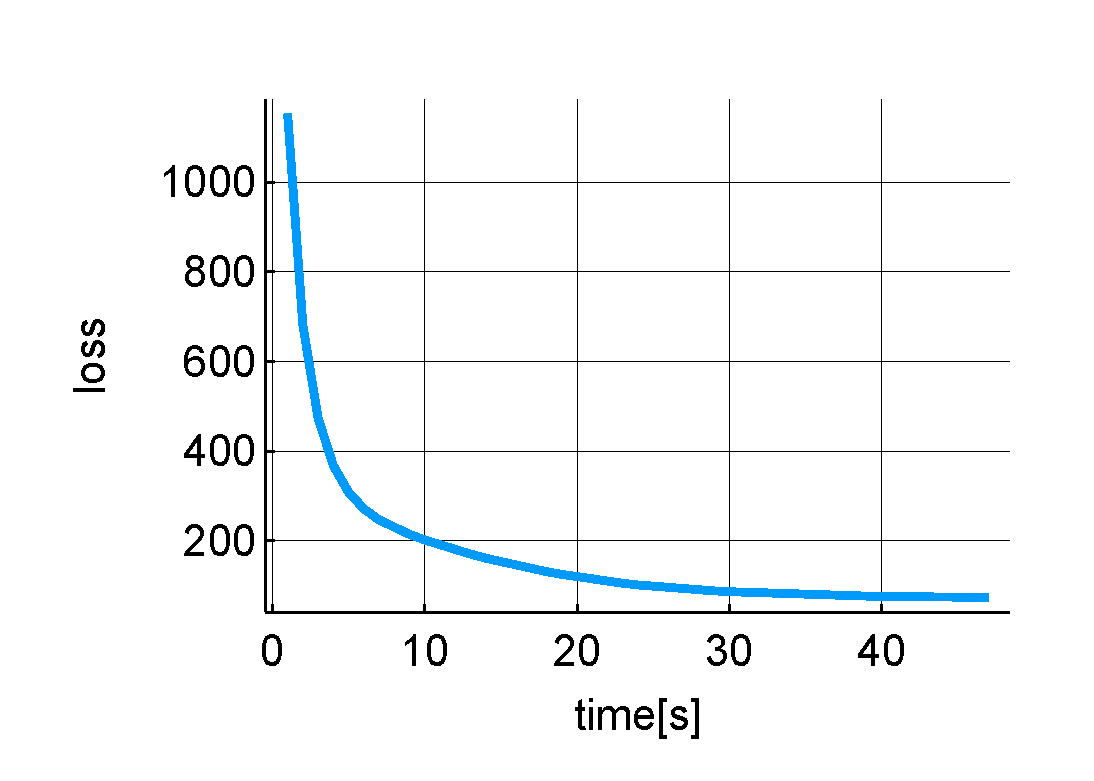
\includegraphics[width=8.0cm]{plots/Images/NCE_loss} }}%
	\subfloat[Comparison of true and estimated pdf]
	{{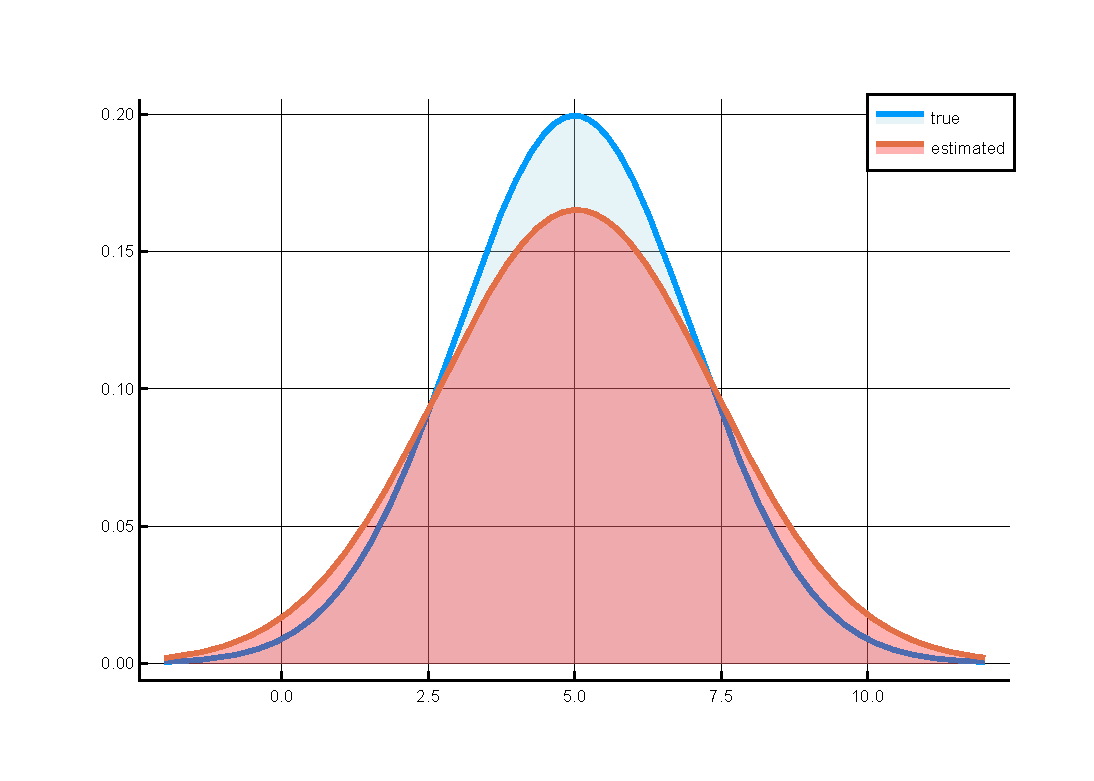
\includegraphics[width=8.0cm]{plots/Images/NCE_results.pdf} }}%
	\caption{Results of the NCE experiment}%
	\label{ggm}%
\end{figure}
\end{example}

\section{Hybrid Dicriminative and Generative Models, HDGM}
In this section will be discussed an approach, how to combine both of the already mentioned models.
Authors of the article \cite{HDGEmain} proposed a solution, however the rationale of this objective originates from \cite{generativevsdisriminative}, where authors show that hybrid models can out--perform purely generative or purely discriminative counterparts.\\
The primary goal is to train a model that can classify $\boldsymbol{x}$ to classes $y$. Secondarily, learned models should be capable of out-of-distribution detection and serve as a generative model. To achieve these goals, a hybrid model consists of a discriminative conditional and a generative conditional by maximizing the sum of both conditional log-likelihoods
\begin{equation}\label{q1q2}
	\min_{\boldsymbol{\theta}}- \mathbb{E}_{p_{\mathrm{data}}(\boldsymbol{x},y)}\left[\log q_{\boldsymbol{\theta}}\left(y|\boldsymbol{x}\right)+ \log q_{\boldsymbol{\theta}}\left(\boldsymbol{x}|y\right) \right],
\end{equation}
where the first term 
\begin{equation}
q_{\boldsymbol{\theta}}\left(y|\boldsymbol{x}\right) = \frac{\exp\left({f_{\boldsymbol{\theta}}\left(\boldsymbol{x}\right)[y]}\right)}{\sum_{i=1}^C\exp\left({f_{\boldsymbol{\theta}}\left(\boldsymbol{x}\right)[y_i]}\right)}
\end{equation}

is a standard Softmax neural net classifier (as mentioned in Equation \eqref{softmax}) and the second term 
\begin{equation}
	q_{\boldsymbol{\theta}}\left(\boldsymbol{x}|y\right) = \frac{\exp\left({f_{\boldsymbol{\theta}}\left(\boldsymbol{x}\right)[y]}\right)}{\sum_{j=1}^N\exp\left({f_{\boldsymbol{\theta}}\left(\boldsymbol{x}_j\right)[y]}\right)},
\end{equation}
is a contrastive loss \eqref{eq:contrastive} attributed a label. This objective  often struggles with the unknown partition function $\sum_{j=1}^N\exp\left({f_{\boldsymbol{\theta}}\left({\boldsymbol{x}_j}\right)[y]}\right)$, which is often intractable, specifically if the number of datapoints is very high. This obstacle is typically addressed using an approximation 
\begin{align}\label{approxcontrasstive}
	&\mathbb{E}_{p_{\mathrm{data}}(\boldsymbol{x},y)}\left[ \log q_{\boldsymbol{\theta}}\left(\boldsymbol{x}|y\right) \right] \\
	&=\mathbb{E}_{p_{\mathrm{data}}(\boldsymbol{x},y)}\left[\log \frac{\exp\left({f_{\boldsymbol{\theta}}\left(\boldsymbol{x}\right)[y]}\right)}{\sum_{j=1}^N\exp\left({f_{\boldsymbol{\theta}}\left(\boldsymbol{x}_j\right)[y]}\right)} \right]  \\
	&\approx\mathbb{E}_{p_{\mathrm{data}}(\boldsymbol{x},y)}\left[\log \frac{\exp\left({f_{\boldsymbol{\theta}}\left(\boldsymbol{x}\right)[y]}\right)}{\sum_{j=1}^M\exp\left({f_\theta\left(\boldsymbol{x}_j\right)[y]}\right)} \right],
\end{align}
where $M < N$ denotes the number of normalization samples. In order to have an sufficient approximation, $M$ has to be sufficiently large - becoming exact in the limit $M \to N$. In practice, increasing $M$ is not simple as it requires a larger memory. However, that does not apply to our experiments. \\
Now it is possible to substitute approximation \eqref{approxcontrasstive} to Equation \eqref{q1q2} that gives a hybrid combination of supervised learning and constrastive learning in the form
\begin{align}\label{eq:q1q2final}
	&\min_{\boldsymbol{\theta}}- \mathbb{E}_{p_{\mathrm{data}}(\boldsymbol{x},y)}\left[\alpha\log q_{\boldsymbol{\theta}}\left(y|\boldsymbol{x}\right)+ \left(1-\alpha\right)\log q_{\boldsymbol{\theta}}\left(\boldsymbol{x}|y\right) \right]  \\
	&\label{eq:hybrid}\approx	\min_{\boldsymbol{\theta}}- \mathbb{E}_{p_{\mathrm{data}}(\boldsymbol{x},y)}\left[\alpha\log \frac{\exp\left({f_{\boldsymbol{\theta}}\left(\boldsymbol{x}\right)[y]}\right)}{\sum_{i=1}^C\exp\left({f_{\boldsymbol{\theta}}\left(\boldsymbol{x}\right)[y_i]}\right)}+ \left(1-\alpha\right)\log \frac{\exp\left({f_{\boldsymbol{\theta}}\left(\boldsymbol{x}\right)[y]}\right)}{\sum_{i=1}^M\exp\left({f_{\boldsymbol{\theta}}\left(\boldsymbol{x}_i\right)[y]}\right)} \right]. 
\end{align}
Parameter $\alpha$ is a weight between $\left[0,1\right]$. It is obvious that in the case of $\alpha = 1$, the objective reduces to the standard cross entropy loss, while $\alpha = 0$, the objective is reduced to a case called an \emph{end-to-end supervised version of contrastive learning}. The choice of parameter $\alpha$ is a decision of the experiment designer, however authors in \cite{HDGEmain} evaluated many possible variants in performed experiments and found out that the choice of $\alpha=0.5$ yields to the highest performance on a classification accuracy. As far as we know, these experiments involved only image classification, unfortunately. \\
Hybrid combination of supervised learning and contrastive learning \eqref{eq:hybrid} is for us absolutely crucial as we extend this approach to multiple instance learning problem, but this is discussed more in further sections.  


\section{Toy problem - Polynomial Regression}
At first, we would like to try out hybrid discriminative and generative approach on simple example before we head into more difficult cases. The goal is to train a model of the form \eqref{eq:hybrid} that was derived in previous section.\\
Assume data $\left\lbrace x_i,y_i \right\rbrace_{i=1}^N$, where $x_i,y_i\in \R$, therefore this is only 2-dimensional problem.  According to energy--based models \ref{EBM}, we know that for joint distribution it holds
\begin{equation}
	p(x,y) = \frac{\exp{\left(f_{\boldsymbol{\theta}}(x)[y]\right)}}{Z(\boldsymbol{\theta})},
\end{equation}
where the model model is given by 
\begin{equation}
	f_{\boldsymbol{\theta}}(x)[y] = -E_{\boldsymbol{\theta}}(x,y) .
\end{equation}
At this point, we should transform our problem to the polynomial regression. We need to be aware of the discriminative term in the Equation \eqref{q1q2}, because we do not want to classify, but we would like to find the best fit to the given data. For this reason, we replace that with the typical regression loss
\begin{equation}\label{S(theta)}
	S = S(\boldsymbol{\theta}) = \sum_{k=1}^N \left(y_k - \sum_{i=0}^{s-1} \theta_i x^i_k\right)^2.
\end{equation}	
Any joint probability distribution can be break down into parts via chain-rule 
\begin{equation}\label{eq:chainrule}
	p(x,y) =	p(y,x) = p(y\vert x)\cdot p(x),
\end{equation}
thus we need to find $p(y\vert x)$ and $p(x)$. From polynomial regression we can obtain conditional probability density 
\begin{equation}\label{eq:linregpdf}
	p(y\vert x, \boldsymbol{\theta}) = \pazocal{N}\left(\sum_{i=0}^{s-1} \theta_i x^i, \sigma^2 \right),
\end{equation}
where symbol $\pazocal{N}(\cdot)$ denotes probability density function of Normal distribution and $\sigma^2$ is known variance. In this case, we also need to determine prior distribution on $x$. To keep this example simple, let the pdf takes the form
\begin{equation}\label{eq:tauprior}
	p(x|\tau) = \pazocal{N}\left(0, \tau^2\right),
\end{equation}
where the choice of parameter $\tau$ is based on the fact that we would like to have a non--informative prior, thus $\tau$ should be adequately high. If the value of $\tau$ is high, data are spread very far from their expected value.  Subtituting Equation \eqref{eq:tauprior} and \eqref{eq:linregpdf} to the \eqref{eq:chainrule} results to
\begin{equation}
	p(x,y) = \pazocal{N}\left(0,\tau^2\right) \cdot \pazocal{N}\left(\sum_{i=0}^{s-1} \theta_i x^i, \sigma^2 \right)  =  \frac{1}{2\pi\sigma\tau}\exp\left(-\frac{\left(y-\sum_{i=0}^{s-1} \theta_i x^i\right)^2}{2\sigma^2}-\frac{x^2}{2\tau^2}\right),
\end{equation}
whereas our desirable model is given by
\begin{equation}\label{modelflinreg}
	f_{\boldsymbol{\theta}}(x)[y] = -\frac{\left(y-\sum_{i=0}^{s-1} \theta_i x^i\right)^2}{2\sigma^2} - \frac{x^2}{2\tau^2}.
\end{equation}
We can now substite \eqref{modelflinreg} and \eqref{S(theta)} into Equation \eqref{q1q2}, yielding
\begin{align}\label{eq:SSEq}
	&\min_{\boldsymbol{\theta}}\Big\lbrace \alpha~S(\boldsymbol{\theta}) - \mathbb{E}_{p_{\mathrm{data}}(x,y)}\left[ \left(1-\alpha\right)\log q_{\boldsymbol{\theta}}\left(x|y\right) \right] \Big\rbrace  =\\
	&\min_{\boldsymbol{\theta}}\Bigg\lbrace \alpha~S(\boldsymbol{\theta}) - \mathbb{E}_{p_{\mathrm{data}}(x,y)}\left[ \left(1-\alpha\right)\log \frac{\exp\left({f_{\boldsymbol{\theta}}\left(x\right)[y]}\right)}{\sum_{i=1}^N\exp\left({f_{\boldsymbol{\theta}}\left(x_i\right)[y]}\right)} \right] \Bigg\rbrace  =\\
	&\min_{\boldsymbol{\theta}}\left\lbrace \alpha~S(\boldsymbol{\theta}) - \mathbb{E}_{p_{\mathrm{data}}(x,y)}\left[ \left(1-\alpha\right)\log \frac{\exp\left({-\frac{\left(y- \sum_{i=0}^{s-1} \theta_i x^i     \right)^2}{2\sigma^2} - \frac{x^2}{2\tau^2}}\right)}{\sum_{k=1}^N\exp\left({-\frac{\left(y-\sum_{i=0}^{s-1} \theta_i x_k^i\right)^2}{2\sigma^2} - \frac{x_k^2}{2\tau^2}}\right)} \right] \right\rbrace.  
\end{align}
Finally, we simplify the generative term $\log q_{\boldsymbol{\theta}}\left(x|y\right)$ into
\begin{equation}
	\log q_{\boldsymbol{\theta}}\left(x|y\right) =  \left(-\frac{\left(y-\sum_{i=0}^{s-1} \theta_i x^i\right)^2}{2\sigma^2} - \frac{x^2}{2\tau^2}\right) - \log \sum_{k=1}^N\exp\left({-\frac{\left(y-\sum_{i=0}^{s-1} \theta_i x_k^i\right)^2}{2\sigma^2} - \frac{x_k^2}{2\tau^2}}\right).
\end{equation}
Note that for $\alpha =1$ we get purely polynomial regression and for $\alpha =0$, the term $S(\boldsymbol{\theta})$ is not involved at all. Now, we have everything we need to perform the experiment.
\subsection{Experiment setup and results}
We would like to test the sensitivity of this approach on the unknown parameter $\tau$ and order of the polynomial $s-1$. In addition, we would like to observe, how the estimated model behaves in relation to $\alpha$. \\
We generated synthetic data, two clusters consisting of 5 datapoints each, then the model was fitted for different weight $\alpha \in \left\{0.0, 0.1, 0.2,\dots,1.0\right\}$, giving 11 different models in total. Models estimated for $\alpha \in \left\{0.0, 0.5, 1.0 \right\}$ are highlighted as they are more important to us then the other models.\\
At first, we trained the mentioned models for the fixed order of the polynomial, but for 6 different values of the parameter $\tau$. Obtained results (Figure \ref{fig:linregtoy_tau}) for small $\tau$ barely vary from those for high $\tau$, that is exactly what we hoped for, since the prior distribution should be non--informative \eqref{eq:tauprior}.  This is very exciting discovery, because there is no need to know much information about the data distribution.\\
Secondly, we trained our polynomial models for the fixed value of $\tau$ with 6 different values of the order of the polynomial. The goal of this part of the experiment is to observe how the contrastive part of Equation \eqref{eq:SSEq} affects the polynomial regression loss for different values of $s-1$. As can be seen in Figure \ref{fig:linregtoy_s}, for small $s-1$, such as $s-1 = 2$, term $\log q_{\theta}\left(x|y\right)$ does not affect polynomial regression too much. However, we get considerable difference for higher orders of the polynomial. Furthermore, it seems that the curve $\alpha = 0$ prefers not to oscillate. This also could be very interesting, because combining of discriminative and generative models could result in better model predictions.    

\begin{figure}[h] 
	\centering
	\subfloat[Estimated model for $\tau=1$ and $s=11$.]
	{{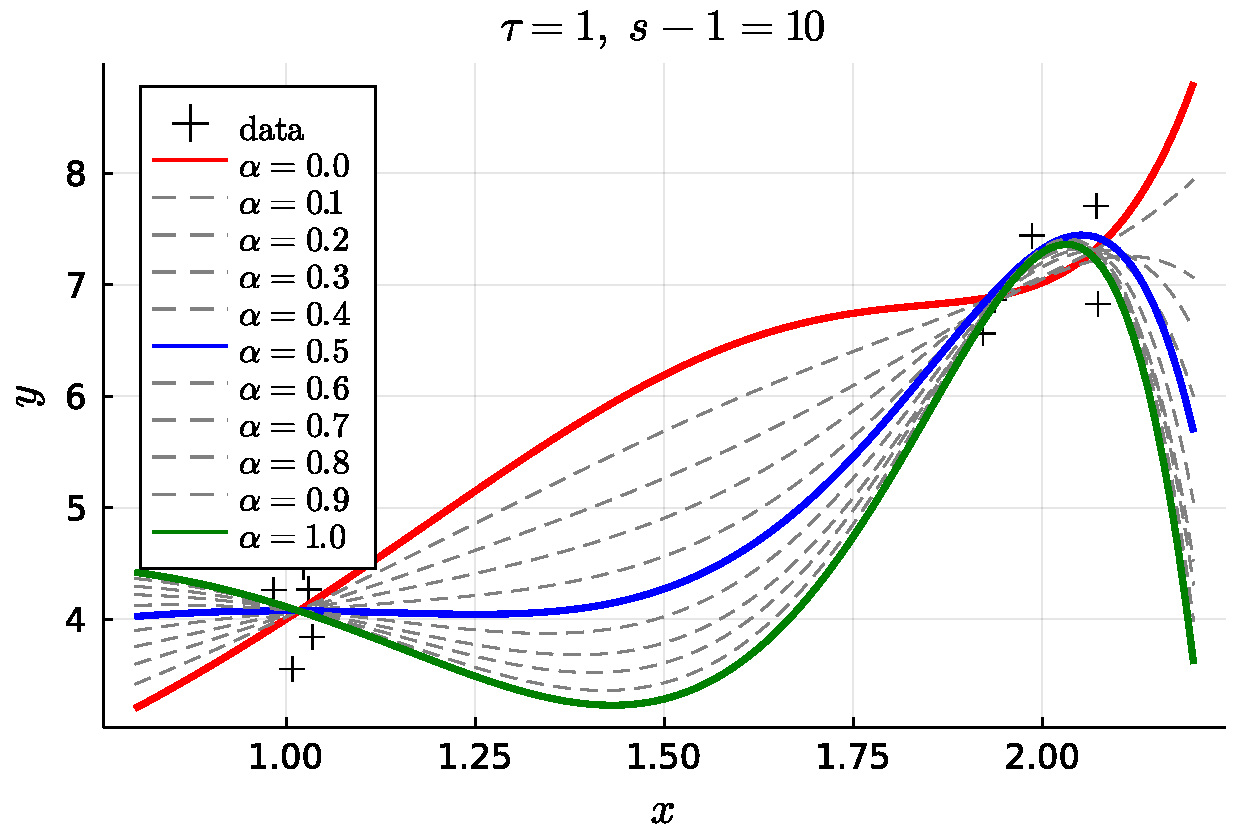
\includegraphics[width=8.0cm]{plots/Images/tau1.pdf} }}%
	\subfloat[Estimated model for $\tau=10$ and $s=11$.]
	{{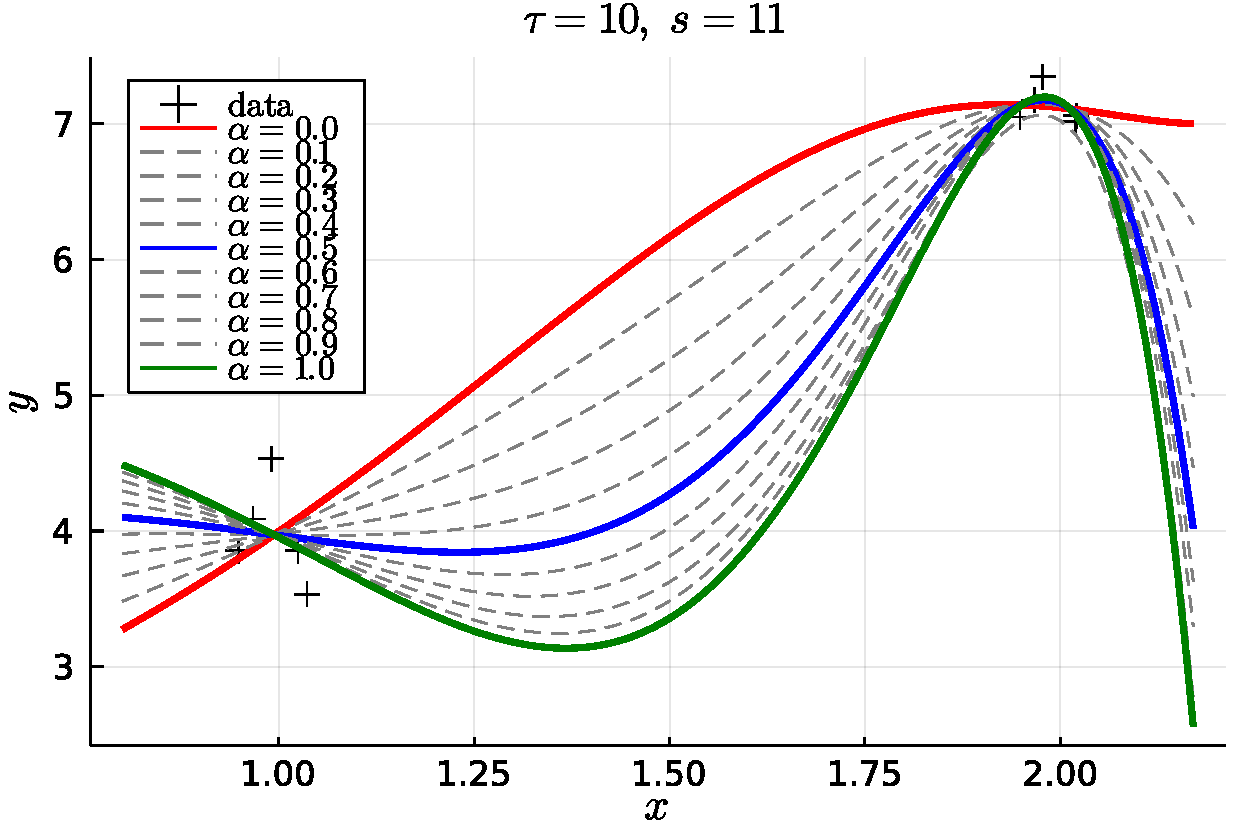
\includegraphics[width=8.0cm]{plots/Images/tau10.pdf} }}%
	\
	\subfloat[Estimated model for $\tau=100$ and $s=11$.]
	{{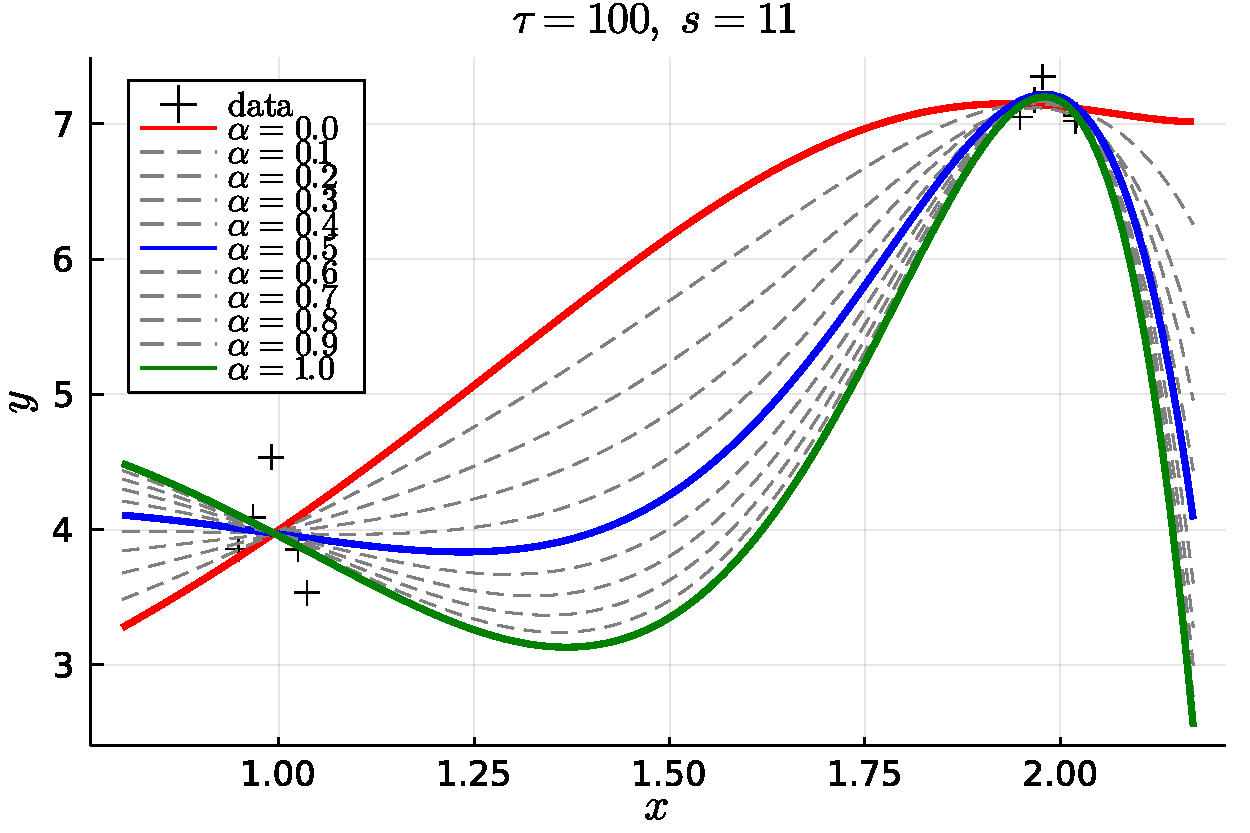
\includegraphics[width=8.0cm]{plots/Images/tau100.pdf} }}%,
	\subfloat[Estimated model for $\tau=1000$ and $s=11$.]
	{{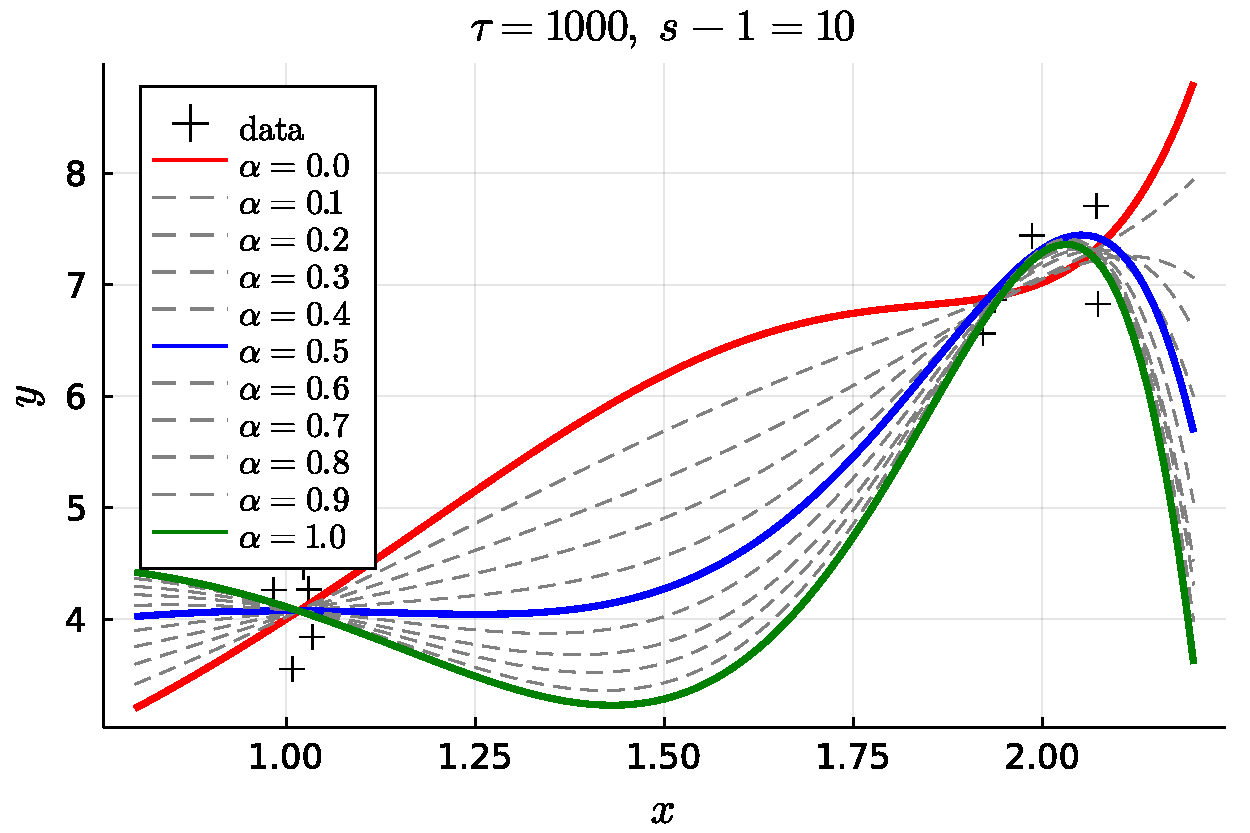
\includegraphics[width=8.0cm]{plots/Images/tau1000.pdf} }}%
	\
	\subfloat[Estimated model for $\tau=100000$ and $s=11$.]
	{{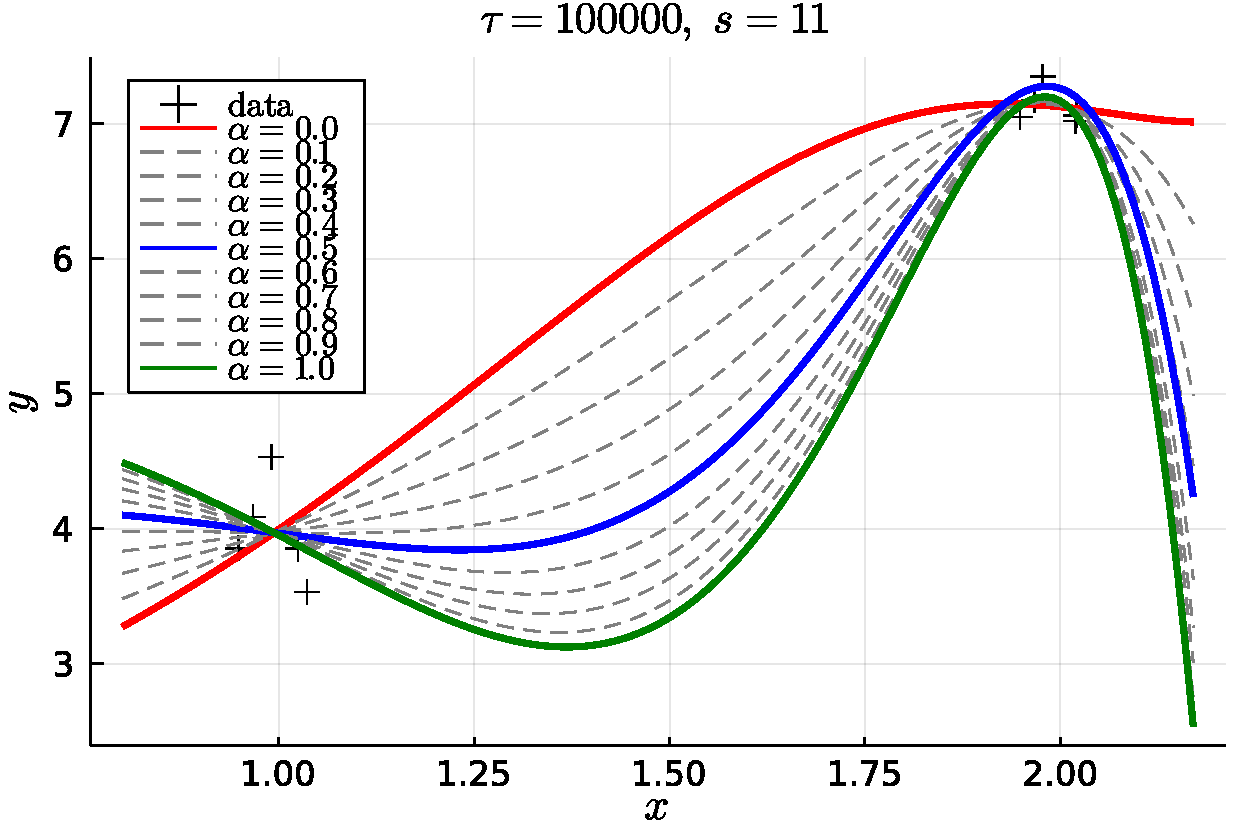
\includegraphics[width=8.0cm]{plots/Images/tau100000.pdf} }}%,
	\subfloat[Estimated model for $\tau=1000000$ and $s=11$.]
	{{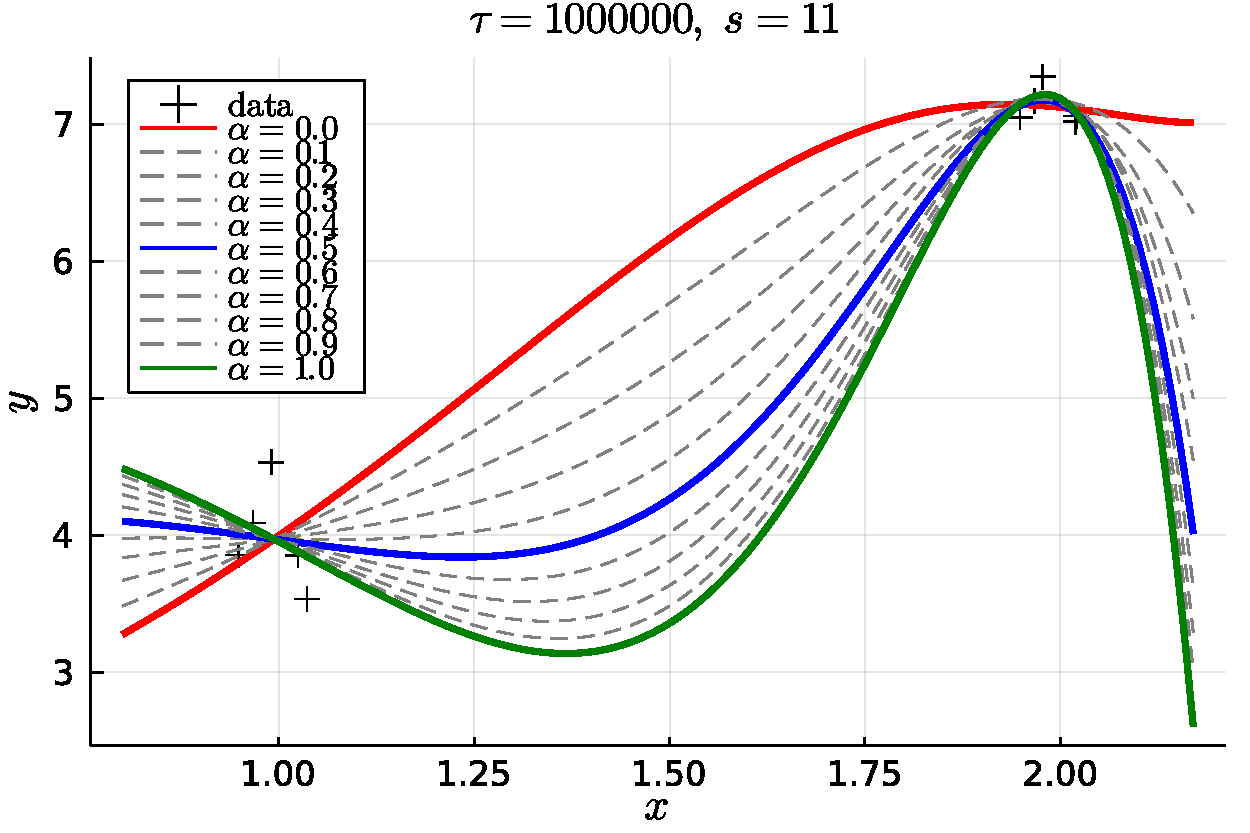
\includegraphics[width=8.0cm]{plots/Images/tau1000000.pdf} }}%
	\caption{Sensitivity of the polynomial model to parameter $\tau$ with parameter $s$ held fixed for six different cases.}%
	\label{fig:linregtoy_tau}%
\end{figure}

\begin{figure}[h]
	\centering
	\subfloat[Estimated model for $\tau=100$ and $s-1=2$.]
	{{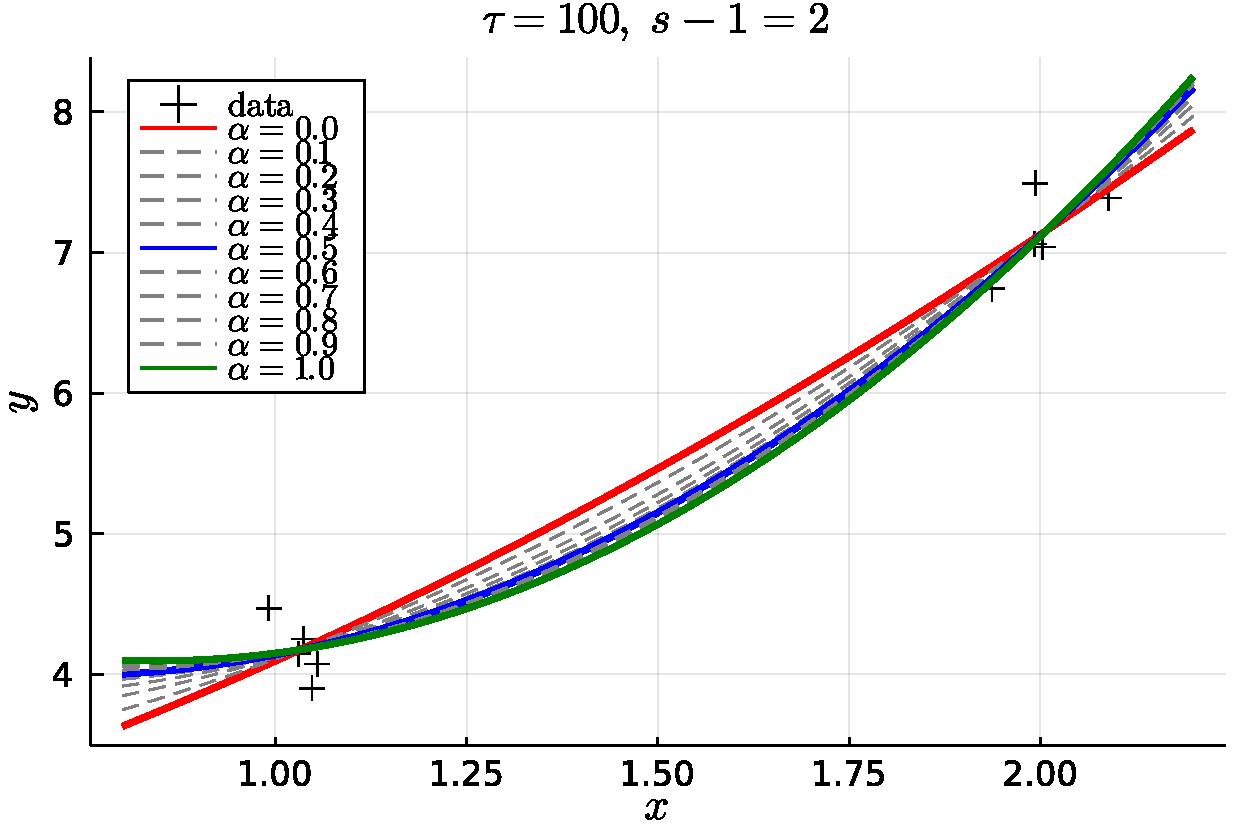
\includegraphics[width=8.0cm]{plots/Images/n2.pdf} }}%
	\subfloat[Estimated model for $\tau=100$ and $s-1=4$.]
	{{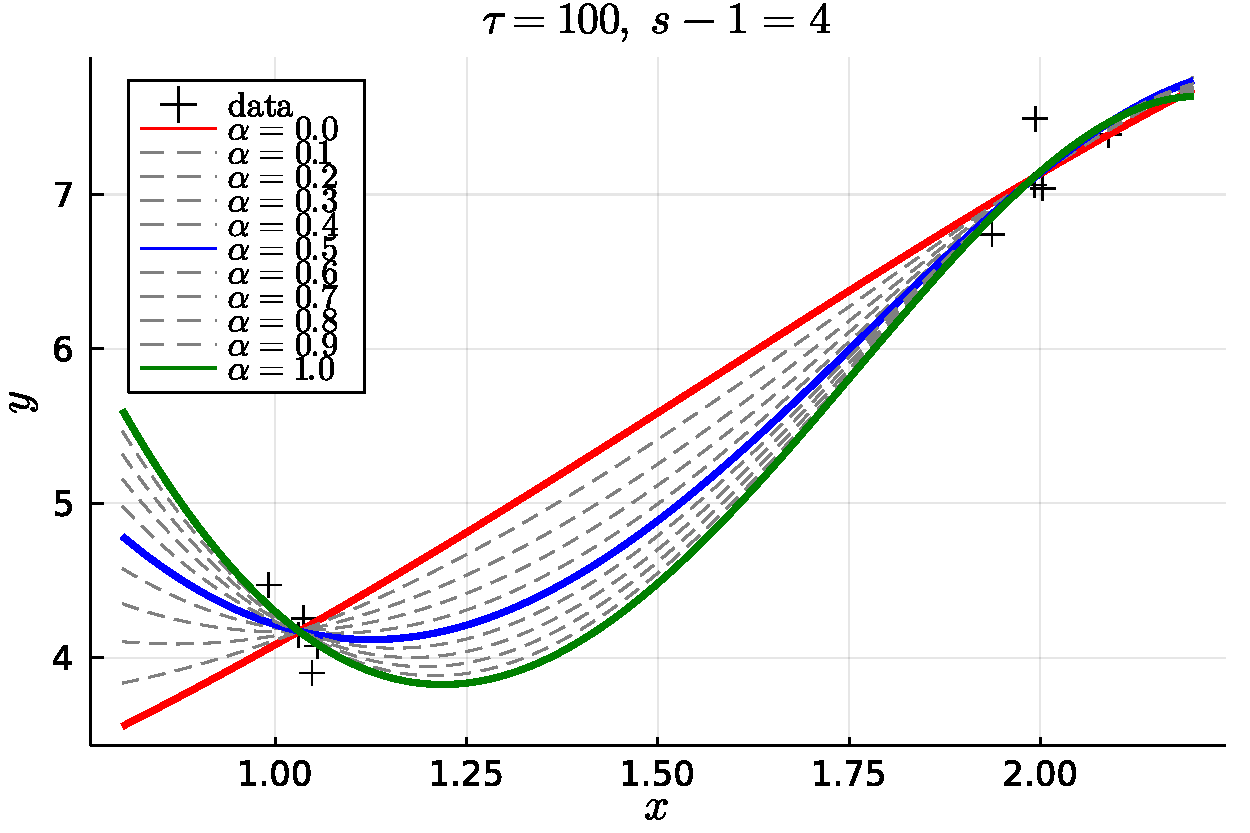
\includegraphics[width=8.0cm]{plots/Images/n4.pdf} }}%
	\
	\subfloat[Estimated model for $\tau=100$ and $s-1=5$.]
	{{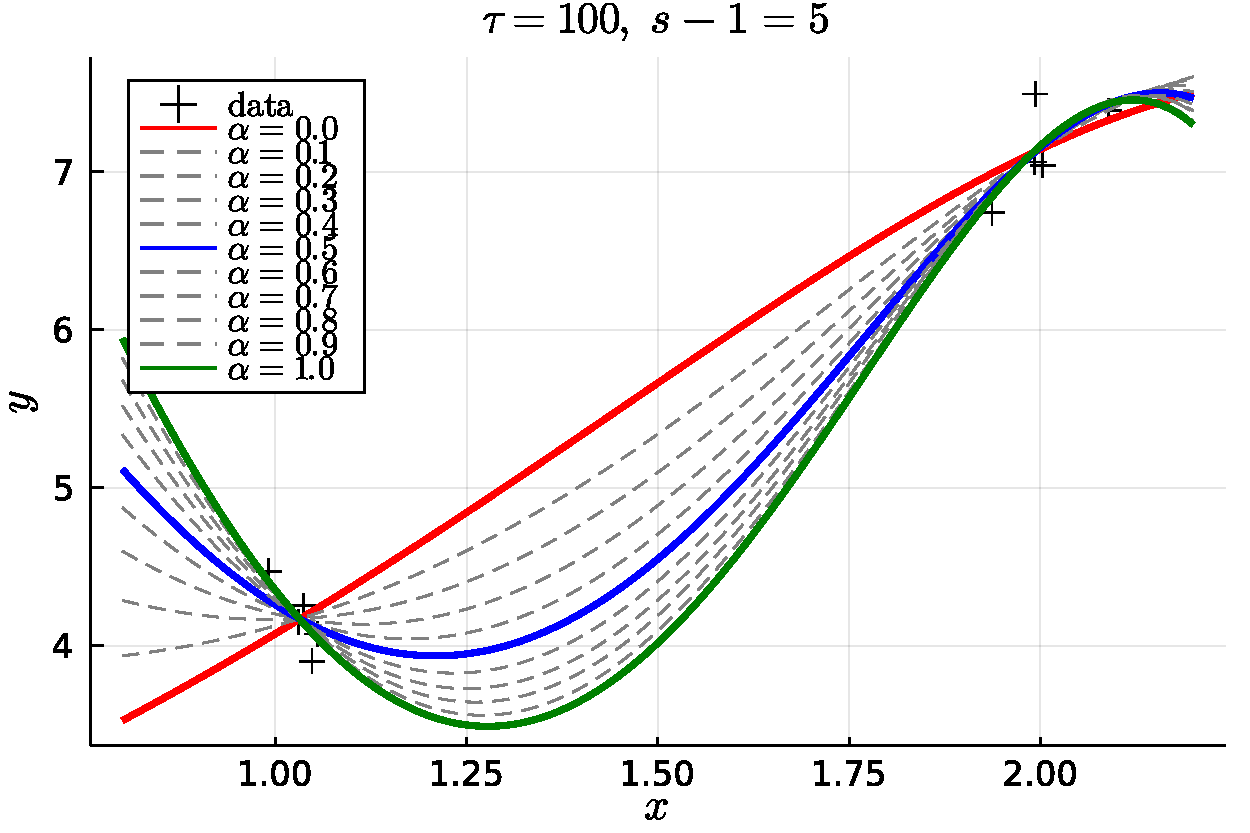
\includegraphics[width=8.0cm]{plots/Images/n5.pdf} }}%,
	\subfloat[Estimated model for $\tau=100$ and $s-1=6$.]
	{{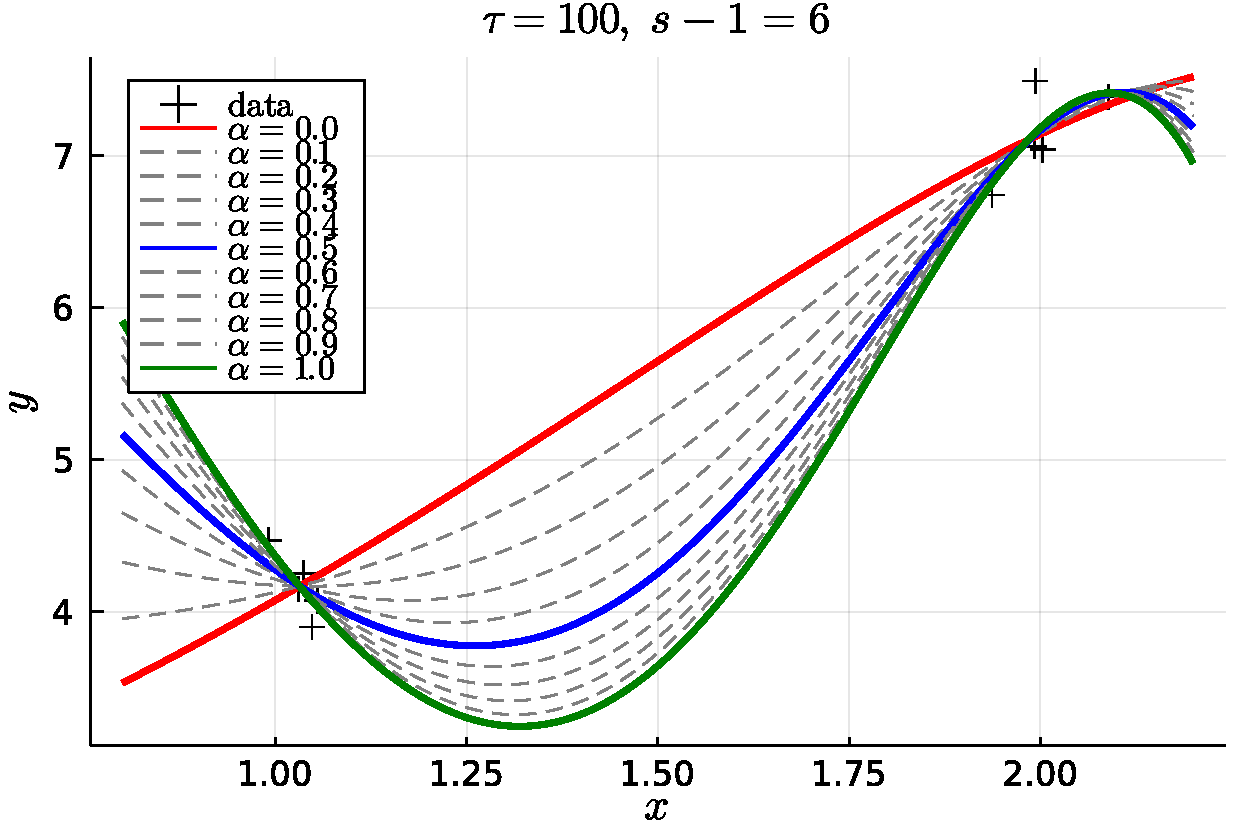
\includegraphics[width=8.0cm]{plots/Images/n6.pdf} }}%
	\
	\subfloat[Estimated model for $\tau=100$ and $s-1=8$.]
	{{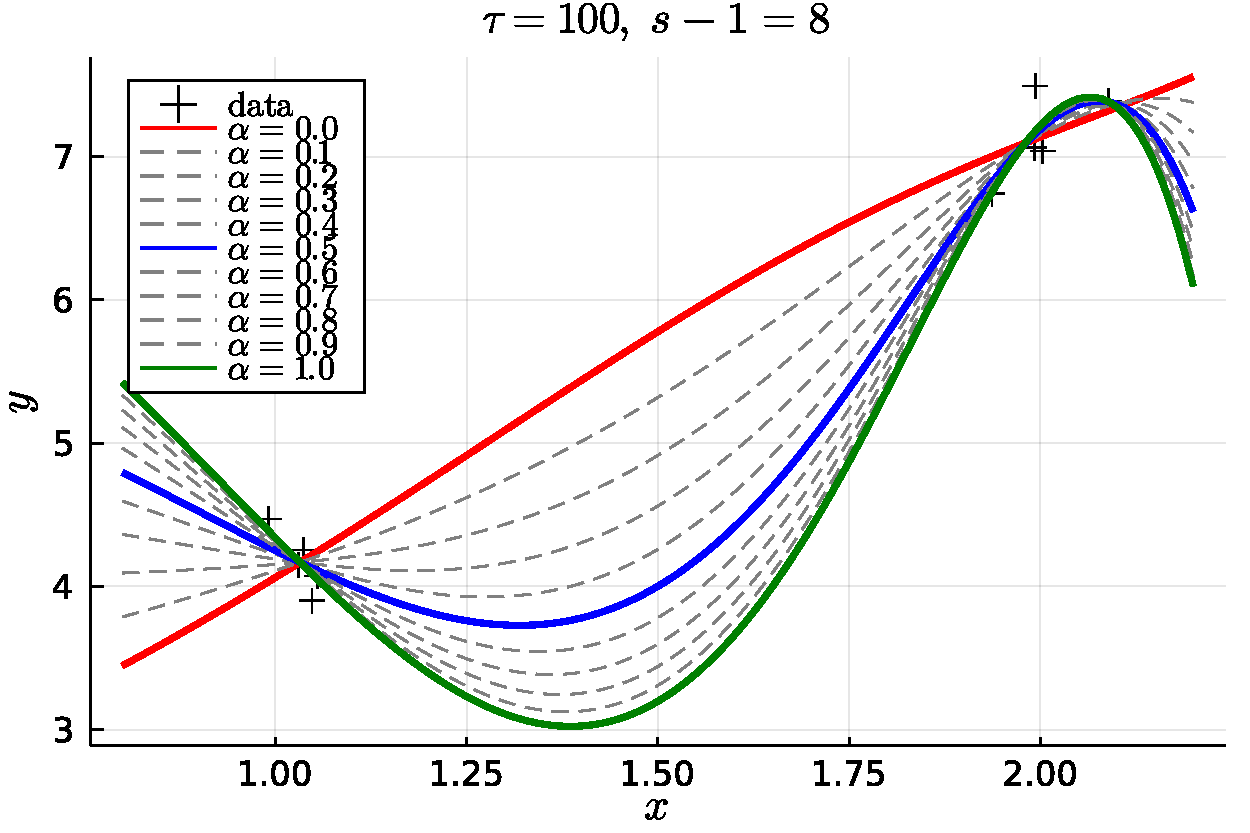
\includegraphics[width=8.0cm]{plots/Images/n8.pdf} }}%,
	\subfloat[Estimated model for $\tau=100$ and $s-1=10$.]
	{{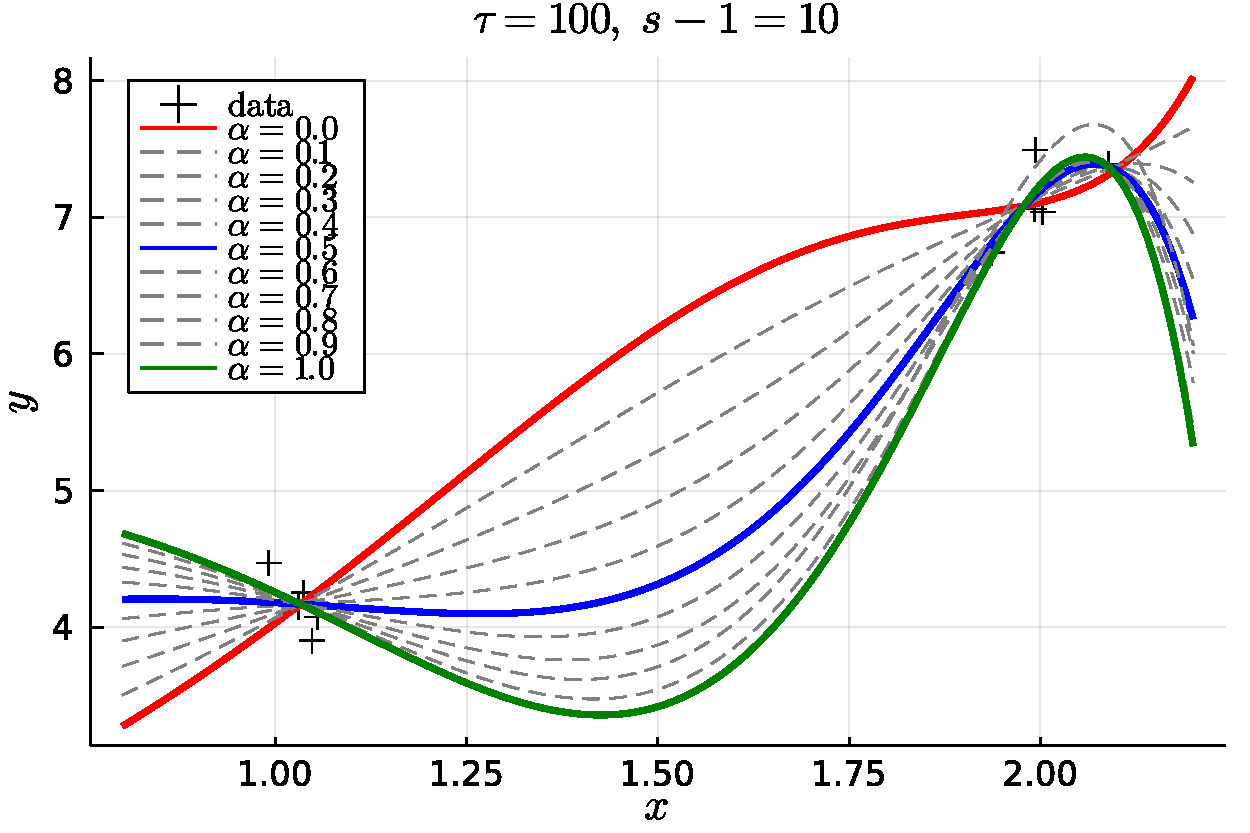
\includegraphics[width=8.0cm]{plots/Images/n10.pdf} }}%
	\caption{Sensitivity of the polynomial model to the order of polynomial $s-1$ for six different cases.}%
	\label{fig:linregtoy_s}%
\end{figure}